\documentclass[rmp,10pt,onecolumn,fleqn,notitlepage]{revtex4-1}

\usepackage{graphicx}
\usepackage{color}
\usepackage{latexsym,amsmath}
\usepackage{physics}
\usepackage{tabularx}
\usepackage{float}
\usepackage{siunitx}
\usepackage{amssymb}
\usepackage{bbold} % to represent identity
\usepackage[caption=false]{subfig} % sfancula la formattazione delle figure se caption è messo su true

% Listing packages
\usepackage{xcolor}
\usepackage{listings}
\usepackage{framed}
\usepackage{inconsolata} % To change the listing font

% URL package and setting
\definecolor{linkcolor}{rgb}{0.65,0.16,0.16}%hyperlink
\usepackage[pdftex,colorlinks=true, pdfstartview=FitV, linkcolor= linkcolor, citecolor= linkcolor, urlcolor= linkcolor, hyperindex=true,hyperfigures=true]{hyperref} %hyperlink%

\usepackage{fancyhdr} % To change page setting

% PAGE SETTING
\pagestyle{fancyplain}
\fancyhf{}
\fancyfoot[R]{\thepage}
\fancyfoot[L]{\today}
\fancyhead[L]{\textbf{Week 10 Report, Quantum Information and Computing (2020)}}
\fancyhead[R]{\textbf{Alice Pagano}}
\renewcommand{\headrulewidth}{0.1pt}
\renewcommand{\footrulewidth}{0.1pt}

% LISTING SETTINGS
\definecolor{cadmiumred}{rgb}{0.89, 0.0, 0.13}
\definecolor{codegray}{rgb}{0.5,0.5,0.5}
\definecolor{commentcolour}{rgb}{0.43,0.63,0.65}
\definecolor{darkgreen}{rgb}{0.0, 0.5, 0.0}

\lstdefinestyle{Fortran}{language=Fortran,
    backgroundcolor=\color{white},
    commentstyle=\color{commentcolour},
    keywordstyle=\bfseries\color{cadmiumred},
    numberstyle=\tiny\color{codegray},
    stringstyle=\color{darkgreen},
    basicstyle=\ttfamily\footnotesize,
    breakatwhitespace=false,
    breaklines=true,
    captionpos=b,
    keepspaces=true,
    numbers=left,
    numbersep=5pt,
    showspaces=false,
    showstringspaces=false,
    showtabs=false,
    tabsize=2,
    frame=single,
    framexleftmargin=11pt,
    %rulecolor=\color{cadmiumred}
}
%\lstset{style=Fortran}

\lstdefinestyle{Gnuplot}{
    backgroundcolor=\color{white},
    commentstyle=\color{commentcolour},
    basicstyle=\ttfamily\footnotesize,
    breakatwhitespace=false,
    breaklines=true,
    captionpos=b,
    keepspaces=true,
    showspaces=false,
    showstringspaces=false,
    showtabs=false,
    tabsize=2,
    frame=single,
    framexleftmargin=11pt,
    rulecolor=\color{cadmiumred}
}

\lstdefinestyle{Python}{language=Python,
    backgroundcolor=\color{white},
    commentstyle=\color{commentcolour},
    keywordstyle=\color{darkgreen},
    numberstyle=\tiny\color{codegray},
    stringstyle=\color{cadmiumred},
    basicstyle=\ttfamily\footnotesize,
    breakatwhitespace=false,
    breaklines=true,
    captionpos=b,
    keepspaces=true,
    numbers=left,
    numbersep=5pt,
    showspaces=false,
    showstringspaces=false,
    showtabs=false,
    tabsize=2,
    frame=single,
    framexleftmargin=11pt
}

% BIBLIOGRAPHY FILE AND SETTING
\begin{filecontents*}{\jobname.bib}
    @article{cite1,
      title={Error handling in Fortran 2003},
      author={Koen Poppe and Ronald Cools and Bart Vandewoestyne},
      journal={ACM Sigplan Fortran Forum},
      year={2012},
      volume={31},
      pages={7-19}
    }
\end{filecontents*}

\bibliographystyle{aipnum4-1}
\setcitestyle{numbers,square}


% Highilight formulas
\newcommand{\mathcolorbox}[2]{\colorbox{#1}{$\displaystyle #2$}}
\newcommand{\hlfancy}[2]{\sethlcolor{#1}\hl{#2}}





\begin{document}



\title{Week 10: Real-space Renormalization Group Algorithm}
\author{Alice Pagano}
\date{\today}

\begin{abstract}
In this Report, given the quantum Ising Hamiltonian in transverse field on a one-dimensional lattice with nearest neighbour interaction, we compute the ground state energy as a function of the transverse field \( \lambda  \) by means of the real-space RG algorithm.
\end{abstract}

\maketitle


\section{Theory}

\subsection{Quantum Ising Model}

The \textbf{quantum Ising model} represents one of the simplest nontrivial many-body quantum system. Let us consider a linear chain of $N$ interacting spins $1/2$ in presence of an external field of \emph{intensity} $\lambda$. The Hamiltonian of the model reads:
\begin{equation}
  \hat{H}_N  = \sum_{i=1}^{N-1} \hat{H}_{i,i+1} = \lambda \sum_{i=1}^{N} \sigma _i^{z} + \sum_{i=1}^{N-1} \sigma _{i}^{x} \sigma _{i+1}^{x}
  \label{eq:hamiltonian}
\end{equation}
where \( \sigma  \)s are the Pauli matrices and the coefficient $\lambda$ determines the relative strength of the external field compared to the nearest neighbour interaction.

In order to solve with numerical simulation this model, let us remind that the Pauli matrices can be rewritten in an explicit form as:
\begin{subequations}
\begin{align}
 \sigma _i^z  &= \mathbb{1}_1 \otimes \mathbb{1}_2 \otimes \dots \otimes \sigma _i^z \otimes \dots \otimes \mathbb{1}_N \label{eq:rel_sigma_z}\\
\sigma _{i}^x \sigma _{i+1}^x &= \mathbb{1}_1 \otimes \mathbb{1}_2 \otimes \dots \otimes \sigma _i^x \otimes \sigma _{i+1}^x \otimes \dots \otimes \mathbb{1}_N\label{eq:rel_sigma_x}
\end{align}
\end{subequations}


\subsection{Real-space Renormalization Group Algorithm}

\textbf{Real-space renormalization group} (RG) method is an approximation method based on a very powerful physical intuition: the hypothesis that the ground state of a system is composed of low-energy states of the system’s (non-interacting) bipartitions.
It is an iterative process to build a system, or a description of a system, of size $2N$ from a truncated description of system of size $N$. The algorithm, for the Hamiltonian in Eq. \eqref{eq:hamiltonian}, proceed as follows:

\begin{enumerate}

\item Consider a system composed of $N$ sites and build the Hamiltonian \( \hat{H}_N: \mathbb{C}^{d^N} \rightarrow \mathbb{C}^{d^N} \).

\item Construct the Hamiltonian of a system of size \( 2N \) using the Hamiltonian \( \hat{H}_N  \) for each bipartition and the interaction among them, as:
\begin{equation}
   \hat{H} _{2N} = \hat{H}_N \otimes \mathbb{1}_N + \mathbb{1}_N \otimes \hat{H}_N + \hat{H}_{int}
   \label{eq:H2N}
\end{equation}
where \( \hat{H}_{int}  \) can be obtained as \( \hat{H}_{int} =  \hat{A}_N \otimes \hat{B}_N    \) where \( \hat{A} = \mathbb{1}_2 \otimes \sigma ^x \) and \( \hat{B} = \sigma ^x \otimes \mathbb{1}_2  \) are the operator acting on each system bipartition.

\item Diagonalize \( \hat{H}_{2N}  \), finding its eigenvalues and eigenvectors.
Compose a matrix $P$ whose columns are the $2^N$ lowest eigenvectors of \( \hat{H}_{2N}  \).

\item Compute the projected Hamiltonian \( \hat{H}_N^{trunc} = P^\dag \hat{H}_{2N} P  \) as well as any other needed operator representation in the projected space. In particular, the projected operator acting on each system bipartition are \( \hat{A}' = P ^\dag A P  \) and \( \hat{B}' = P ^\dag B P  \).

\item Repeat the steps 1–4 with the following substitutions
\begin{equation*}
  \hat{H}_N \rightarrow  \hat{H}_{N}^{trunc}, \quad A' \rightarrow \hat{A}', \quad B' \rightarrow \hat{B}'
\end{equation*}
until the desired system size is reached or convergence to the renormalization group fixed point is achieved. Notice that, at each step of the algorithm, the dimension of the Hamiltonian representation is kept constant to $N$.

\end{enumerate}

% \subsection{Infinite Density Matrix Renormalization Group Algorithm}
% \textbf{Density Matrix Renormalization Group} (DMRG) method is a powerful modification of the original RG algorithm, where the truncation rule is improved resulting in a higher precision description of the final state at the price of slowing down the growth of the system size.
% In particular, to describe systems with nearest neighbor interaction at the thermodynamical limit (\textbf{infinite DMRG}), the algorithm proceed as follows:
%
% \begin{enumerate}
% \item Consider a system of size \( N \) such that \( \mathcal{H}_N : \mathbb{C}^{d^N} \rightarrow \mathbb{C}^{d^N} \).  Regroup the $N$ sites in 2 single sites in the middle and others in two groups of $M$ sites. The system Hamiltonian can be written as:
% \begin{equation}
%     \hat{H} _N = \hat{H}_{L+1} + \hat{H}_{int} + \hat{H}_{R+1}
%   \label{eq:DMRG_H}
% \end{equation}
% where \( \hat{H}_{L+1} \) and \( \hat{H}_{R+1} \) are referred at as the left and right enlarged blocks, and \( \hat{H}_{int} \) is the interaction among them. The dimension of the Hilbert space of the system is $(dm)^2$, where $m = d^M$ is the dimension of the $M$ grouped sites.
%
% \item Diagonalize \( \hat{H}_N  \) such that the ground state can be expressed as:
% \begin{equation}
%   \ket{E_0^N} = \sum_{ }^{}  \psi_{\beta _1, \beta _2} \ket{\beta _1} \ket{\beta _2}
%   \label{eq:DMRH_ground_state}
% \end{equation}
% where \( \beta _i = 1, \dots, d^{M+1}  \).
%
% \item Compute the density matrix of the ground state \( \rho _0^N = \ketbra{E_0^N}{E_0^N}  \) and the reduced density matrix of one half of the system \( \rho _L = \Tr_R \rho _0^N \).
%
% \item  Diagonalize \( \rho _L = \sum_{i=1}^{md}  w_i \ketbra{w_i}{w_i}   \) and define the projector $P = \sum_{i=1}^m \ketbra{w_i}{w_i} $ whose columns are the \( 2^m \) eigenvectors of \( \rho _L \) with higher eigenvalue.
%
% \item Project the Hamiltonian \( \hat{H}_L^{trunc}=P ^\dag \hat{H}_L P   \) and the operator \( \hat{H}_{int}' =  P ^\dag \hat{H}_{int } P   \). We obtain an effective matrix describing the Hamiltonian for the system of $N$ sites of dimension $m$ instead than $md$.
%
% \item Repeat the steps 1–5 with the following substitutions
% \begin{equation*}
%   \hat{H}_N \rightarrow  \hat{H}_{N}^{trunc}
% \end{equation*}
% until the desired system size is reached or convergence to the renormalization group fixed point is achieved. Notice that, at each step of the algorithm, the dimension of the Hamiltonian representation is incremented by two sites while keeping the computational resources constant.
% \end{enumerate}


\clearpage



\section{Code Development}

In order to write the hamiltonian of the Ising model for a system with $N$ particles and compute its ground state by means of the RG algorithm, we develop a Fortran program.

First of all, a user-defined \texttt{FUNCTION} {\bfseries\texttt{tensor$\_$product}}\texttt{(Mat1,Mat2)} is coded for performing the tensor product between two matrices (i.e. between operators) \texttt{Mat1} and \texttt{Mat2}.
Then, the main steps of the program are:
\begin{enumerate}

\item The total number of subsystems \texttt{N} and the number of iterations of the RG algorithm \texttt{iter} are given as input. Subsequently, we also create an array of \( \lambda \) values in the range $[-5;5]$ and we define the matrices \( \sigma _x \) and \( \sigma _z \).

\item Then, we loop over the values of \( \lambda  \). For each \( \lambda  \), we initilize the system hamiltonian as the sum between a non-interacting term \texttt{H$\_$non$\_$int} and an interacting one \texttt{H$\_$int}. In particular, the two terms are computed by calling:
        \begin{itemize}

        \item the \texttt{FUNCTION} {\bfseries\texttt{H$\_$non$\_$int}}\texttt{(N,sigmaz)}, which takes in input the number of particles and \( \sigma _z \). It performs the tensor product between \( \sigma _z \) and the identity matrix by exploiting the relationship given by Eq. \eqref{eq:rel_sigma_z}.

        \item the \texttt{FUNCTION} {\bfseries\texttt{H$\_$int}}\texttt{(N,sigmax)}, which takes in input the number of particles and \( \sigma _x \). It performs the tensor product between \( \sigma _x \) and the identity matrix by exploiting the relationship given by Eq. \eqref{eq:rel_sigma_x}.
    \end{itemize}
Moreover, we initilize also the \( A \) and \( B \) operators as the tensor product between the identity matrix and \( \sigma _x \).

\begin{minipage}[t]{0.65\linewidth}%\vspace{0pt}
\begin{lstlisting}[style=Fortran]
! Initialization of system Hamiltonian and of operators
H = lambda(ii)*H_non_int(N_part,sigmaz) + H_int(N_part,sigmax)
A = tensor_product(identity(N_part-1),sigmax)
B = tensor_product(sigmax,identity(N_part-1))\end{lstlisting}
\end{minipage}

\item For each \( \lambda  \) and for \texttt{iter} times, we call \texttt{SUBROUTINE} {\bfseries\texttt{real$\_$space$\_$RG}} \texttt{(HN, N, A, B)} to perform the RG algorithm. First of all, the Hamiltonian of size \( 2N \) is initialized as in Eq. \eqref{eq:H2N}. Then, we diagonalize \( \hat{H} _{2N} \) and we construct the projected matrix \( P \) and its adjoint \( P ^\dag  \). At least, the Hamiltonian \( \hat{H}_{2N}  \) and the operators \( A \) and \( B \) are projected.

\begin{minipage}[t]{0.97\linewidth}%\vspace{0pt}
\begin{lstlisting}[style=Fortran]
subroutine real_space_RG(HN, N, A, B)
    ...
    ! Set dimension
    dim = 2**N

    allocate( H2N(dim**2,dim**2)     )
    allocate( A_int(dim**2 ,dim**2)  )
    allocate( B_int(dim**2 ,dim**2)  )
    allocate( P(dim**2,dim)          )
    allocate( Pdag(dim,dim**2)       )

    ! Initialize H2N Hamiltonian
    H2N = tensor_product(HN, identity(N)) +tensor_product(identity(N), HN) + tensor_product(A,B)

    CALL diag_hamiltonian(H2N, eig_val, eig_vec)

    ! Initialize P and Pdag (adjoint)
    do ii = 1, dim, 1
        P(:,ii) = eig_vec(:,ii)
    end do
    Pdag = transpose(conjg(P))

    ! Update H2N hamiltonian
    HN = matmul(matmul(Pdag, H2N),P)

    ! Update A_int and B_int
    A_int = tensor_product(A,identity(N))
    B_int = tensor_product(identity(N),B)
    A = matmul(matmul(Pdag,A_int),P)
    B = matmul(matmul(Pdag,B_int),P)

end subroutine real_space_RG\end{lstlisting}
\end{minipage}

Moreover, before each iteration, we divide by a 2 factor the Hamiltonian \( H_{N} \) and by \(\sqrt{2}  \) the \( A \) and \( B \) operators in order to keep the numbers low.

\begin{minipage}[t]{0.55\linewidth}%\vspace{0pt}
\begin{lstlisting}[style=Fortran]
! Perform RG algorithm
do jj=1,iter,1
    ! Divide per 2 each cycle to keep the numbers low
    H = H * 0.5
    A = 1/sqrt(2.) * A
    B = 1/sqrt(2.) * B
    ! Call RG algorithm
    CALL real_space_RG(H, N_part, A, B)
end do\end{lstlisting}
\end{minipage}


\item Finally, for each \( \lambda  \), we diagonalize the final Hamiltonian \( \hat{H}_N  \) and we find the ground state energy density \( G_0 = E _0 /N \).
\end{enumerate}

The ground state energy \( G_0 (\lambda ) \) is plotted as a function of \( \lambda \) thanks to a gnuplot script.




\section{Results}

The program is executed for simulating a system of \( N=2 \) particles with the interaction strength varing in the range \( \lambda \in [-5;5] \). More specifically, the RG algorithm is executed for \( N_{iter} = 100 \).

The results of the simulation are illustrated in Fig. \ref{fig:result}.
In this plot, the RG method outcomes are compared with the one of the Mean Field solution:
\begin{equation}
    G_0^{MF} (\lambda ) =
  \begin{cases}
   -1 - \lambda^2/4 & \lambda \in [-2:2] \\
   - \abs{\lambda } & \lambda \not \in [-2:2]
  \end{cases}
\end{equation}
We note that there is a good agreement between the two solutions.


\begin{figure}[h!]
\centering
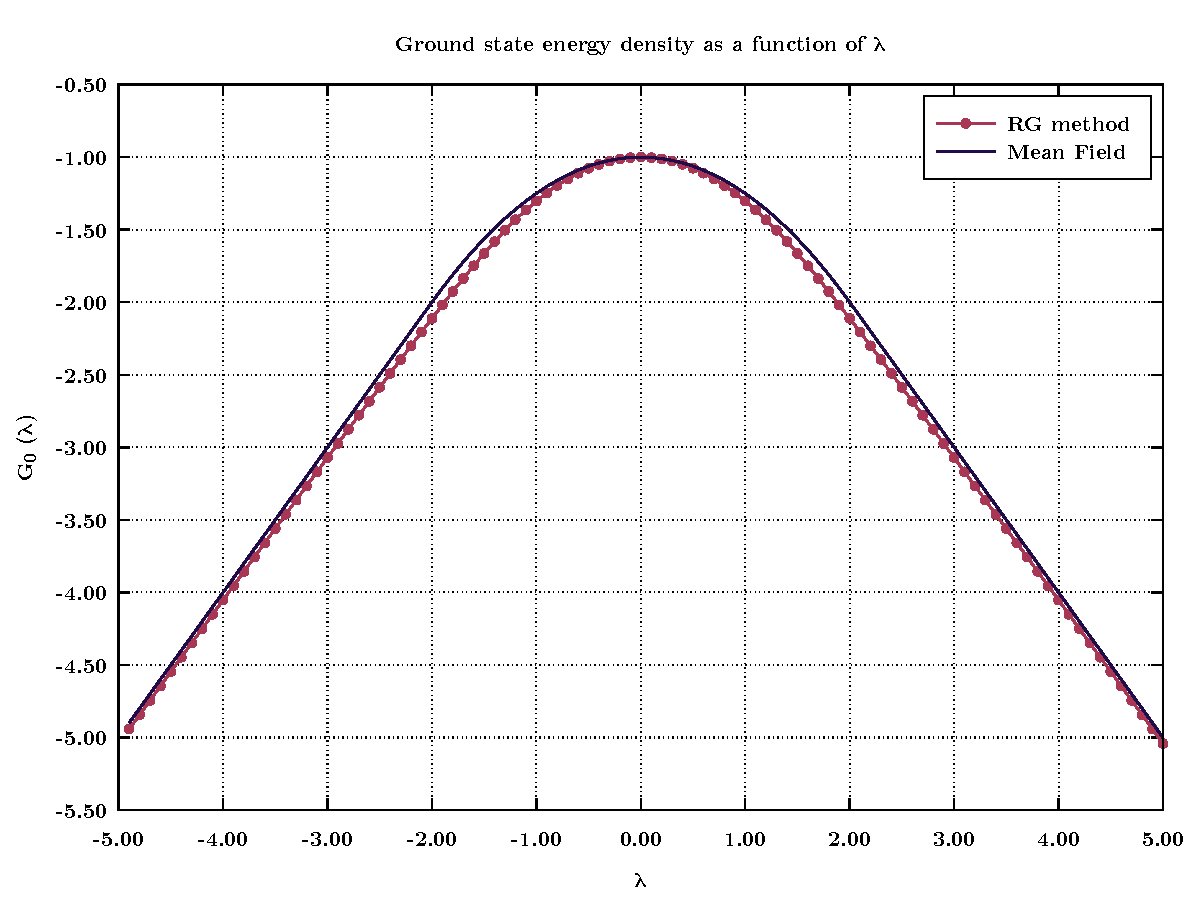
\includegraphics[width=0.7\textwidth]{image/RG_ground_state.pdf}
\caption{\label{fig:result} Ground state energy \( G_0 (\lambda )\) of a quantum Ising model as a function of \( \lambda  \) for \( N=2 \) particles. Both the Mean Field solution and the results of RG algorithm are reported.}
\end{figure}




\section{Self-evaluation}
The code implemented works well and returns consistent results. In particular, we learn how to compute the ground state energy of a quantum Ising model by using the RG algorithm and we study its spectrum for different values of the strength parameters \( \lambda  \). In a further development of the code, it could be useful to compute the error associated to each RG iteration in order to find the optimal iteration number. Moreover, the tensor product function should be optimized to simulate also more complex systems.





\end{document}
